
\begin{figure}[h!]
    \textbf{Tema d'Esame di Gennaio 2016}\\ \\
    Una molla viene compressa di 17 cm prima di lanciare una palla verso un piano inclinato
    senza attrito. La palla ha massa 1kg e il piano inclinato ha un'altezza H=1.28 m. Quanto vale
    la costante elastica della molla affinché la palla arrivi con una velocità di 4 m/s in cima al
    piano ?
    \\
        \begin{center}
            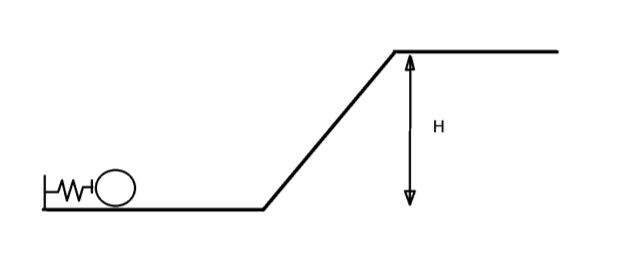
\includegraphics[scale=0.5]{ES2/GEN022016.jpg}
        \end{center}
    \end{figure}
    
    \begin{figure}[h!]
    \textbf{Tema d'Esame di Febbraio 2016}\\ \\
    Una palla di massa $250g$ è lanciata da una molla con costante elastica $63 N/m$ compressa di $45 cm$. La palla viaggia attraverso un piano inclinato alto $72 cm$. Una volta arrivata in cima al piano inclinato la palla incontra una superficie piatta frenante. Il coefficente d'attrito dinamico palla-superficie è di $m=0.42$. Che distanza percorre la palla sulla superficie frenante prima di fermarsi?
    \\
        \begin{center}
            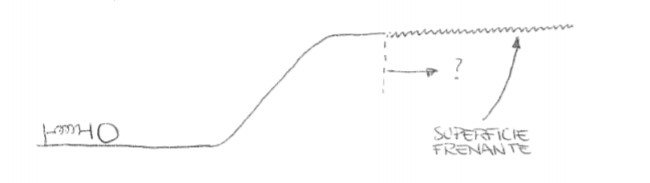
\includegraphics[scale=0.5]{ES2/FEB022016.jpg}
        \end{center}
        \noindent\fbox{
            \parbox{\textwidth}{
                \null\hfill \textbf{Soluzione:} $ s=4.477m $\\
                \textbf{Procedimento: } \\
                Trasformare le unità di misura:\\
                $\Delta x= 45cm =0.45m$\\
                $h=72cm=0.72m$\\ \\
                Impostando il seguente sistema, considerando come punto A la molla , il punto B il punto immediatamente dopo il piano inclinato e il punto C dove la palla si fermerà sul piano scabro.\\
                $$
                \begin{cases}
                    U_{El,A} = U_B + K_B \\
                    U_B + K_B = U_C + L_a
                \end{cases}
                =
                \begin{cases}
                    \frac{1}{2}\cdot k \cdot \Delta x^2 = m\cdot g \cdot h + \frac{1}{2} \cdot m \cdot v^2\\
                    \frac{1}{2}\cdot m \cdot v^2 = \mu_d \cdot m \cdot g \cdot cos(\alpha) \cdot \Delta s
                \end{cases}
                $$
                $$
                \begin{cases}
                    6.378J = 1.766J + 0.125kg \cdot v^2\\
                    0.125kg\cdot v^2 = 103N \cdot \Delta s
                \end{cases}
                =
                \begin{cases}
                    v^2 = 36.896 m^2/s^2 \\
                    \Delta s= 4.477m
                \end{cases}
                $$
                
            }
        }                  
    \end{figure}
    
    \begin{figure}[h!]
    \textbf{Tema d'Esame di Giugno 2016}\\ \\
    Una molla ideale può essere compressa di $1.0 m$ da una forza di $100 N$. La stessa molla è posta alla fine di un piano inclinato con attrito (coefficiente $0.2$) che forma un angolo di 30$^{\circ}$ con l'orizzontale. Una massa $M$ di $10 kg$ viene lasciata cadere da ferma dal vertice del piano inclinato e si arresta momentaneamente dopo aver compresso la molla di $2.0 m$. Qual'è la velocità della massa un attimo prima di toccare la molla? 
    \\
        \begin{center}
            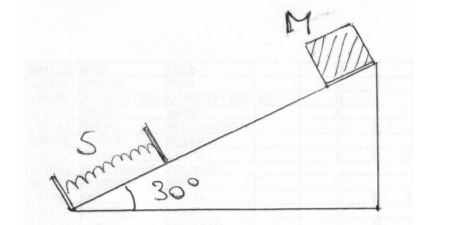
\includegraphics[scale=0.5]{ES2/GIU022016.jpg}
        \end{center}

        \noindent\fbox{
            \parbox{\textwidth}{
                \null\hfill \textbf{Soluzione:} $ s=6.324m/s $\\
                \textbf{Procedimento: } \\
                Trasformare le unità di misura:\\
                $\Delta x= 45cm =0.45m$\\
                $h=72cm=0.72m$\\ \\
                Impostando il seguente sistema, considerando come punto A la molla , il punto B dove parte il corpo.\\
                È conveniente ribaltare la struttura del problema per dire che la massa parte dalla molla e arriva nel punto B con velocità 0.\\
                $$
                \begin{cases}
                    U_{El,A} - L_a= U_B  \\
                    K_A - L_a = U_B
                \end{cases}
                =
                \begin{cases}
                    \frac{1}{2}\cdot k \cdot \Delta x^2 - \mu_d \cdot m \cdot g \cdot cos(\alpha) \cdot \Delta s= m\cdot g \cdot h \\
                    \frac{1}{2}\cdot m \cdot v^2 - \mu_d \cdot m \cdot g \cdot cos(\alpha) \cdot \Delta s=m\cdot g \cdot h
                \end{cases}
                $$
                \textbf{Nota:} con la seconda equazione del sistema ipotizziamo che a prescindere della forza con cui sia stata spinta dalla molla, la velocità necessaria che serve per spingere un corpo su una superficie scabra dovrà essere uguale a tale forza. \\
                A questo punto basta solamente eguagliare:\\
                $\frac{1}{2}\cdot k \cdot \Delta x^2 = \frac{1}{2}\cdot m \cdot v^2 \quad 200J=5kg\cdot v^2 \quad v=\sqrt{40m^2 /s^2}=6.324m/s$\\
                \textbf{Nota:} Questo ragionamento è valido solamente se si ipotizza che la molla posta sul piano inclinato sia stata compressa fino all'origine, (banalmente che abbia energia potenziale $m\cdot g\cdot h$ nulla nel punto A).
               
                
            }
        }    
    \end{figure}
    
    \begin{figure}[h!]
    \textbf{Tema d'Esame di Luglio 2016}\\ \\
    La molla della figura ha una costante elastica $k = 120 \frac{N}{m}$ e una lunghezza a riposo di $45cm$. Quando un blocco di massa $M$ viene attaccato alla molla l'estensione di equilibrio della molla è $60cm$. Il piano inclinato è liscio(senza attrito) e forma un angolo di $40^\circ$ con l'orizzontale. Se la massa viene tirata leggermente verso il basso e viene rilasciata, qual è il periodo di oscillazione? 
    \\
        \begin{center}
            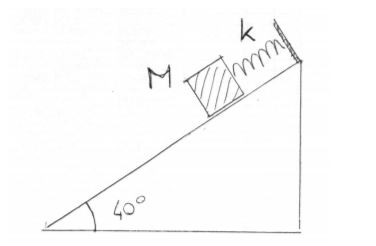
\includegraphics[scale=0.5]{ES2/LUG022016.jpg}
        \end{center}
    \end{figure}
    
    